\documentclass[oneside]{book}
\usepackage[UKenglish]{babel}
\usepackage{graphicx}
\usepackage{natbib}
\usepackage[colorlinks]{hyperref}
\usepackage[dvipsnames]{xcolor}
\usepackage{ amssymb, dsfont }
\usepackage{tikz}
\usepackage{dsfont}

\hypersetup{
  linkcolor  = Magenta,
  citecolor  = Aquamarine,
  urlcolor   = Periwinkle,
  linktoc    = page
}
\usepackage{algorithm}
\usepackage[noend]{algpseudocode}
\usepackage{amsmath,amssymb,bm}

\usepackage{enumitem}
\usepackage{subcaption}
\usepackage{wrapfig}
\usepackage{minted}  % Code embedding in document
\usepackage[none]{hyphenat}

\usepackage{mathtools}
\usepackage{verbatim}

\makeatletter
\newcommand\RedeclareMathOperator{%
  \@ifstar{\def\rmo@s{m}\rmo@redeclare}{\def\rmo@s{o}\rmo@redeclare}%
}
% this is taken from \renew@command
\newcommand\rmo@redeclare[2]{%
  \begingroup \escapechar\m@ne\xdef\@gtempa{{\string#1}}\endgroup
  \expandafter\@ifundefined\@gtempa
     {\@latex@error{\noexpand#1undefined}\@ehc}%
     \relax
  \expandafter\rmo@declmathop\rmo@s{#1}{#2}}
% This is just \@declmathop without \@ifdefinable
\newcommand\rmo@declmathop[3]{%
  \DeclareRobustCommand{#2}{\qopname\newmcodes@#1{#3}}%
}
\@onlypreamble\RedeclareMathOperator
\makeatother

\DeclareMathOperator{\E}{\mathbb{E}}
\DeclareMathOperator{\V}{\mathbb{V}}
\RedeclareMathOperator{\Pr}{\mathbb{P}}
\newcommand{\matr}[1]{\bm{#1}}     % ISO complying version
\newcommand{\vect}[1]{\bm{#1}}     % ISO complying version

\DeclarePairedDelimiter\ceil{\lceil}{\rceil}
\DeclarePairedDelimiter\floor{\lfloor}{\rfloor}

\DeclareMathOperator*{\argmax}{arg\,max}  % in your preamble
\DeclareMathOperator*{\argmin}{arg\,min}  % in your preamble 

\usepackage[nameinlink,noabbrev]{cleveref}
\newcommand*{\fullref}[1]{\hyperref[{#1}]{\Cref*{#1} -- \nameref*{#1}}}

\newcommand{\norm}[1]{\left\lVert#1\right\rVert}


\usepackage[T1]{fontenc}

\usepackage{adjustbox} % Used to constrain images to a maximum size 
\usepackage{xcolor} % Allow colors to be defined
\usepackage{geometry} % Used to adjust the document margins
\usepackage{amsmath} % Equations
\usepackage{amssymb} % Equations
\usepackage{textcomp} % defines textquotesingle
% Hack from http://tex.stackexchange.com/a/47451/13684:
\AtBeginDocument{%
\def\PYZsq{\textquotesingle}% Upright quotes in Pygmentized code
}
\usepackage{upquote} % Upright quotes for verbatim code
\usepackage{eurosym} % defines \euro
\usepackage[mathletters]{ucs} % Extended unicode (utf-8) support
\usepackage[utf8x]{inputenc} % Allow utf-8 characters in the tex document
\usepackage{fancyvrb} % verbatim replacement that allows latex
\usepackage{grffile} % extends the file name processing of package graphics 
% to support a larger range 
% The hyperref package gives us a pdf with properly built
% internal navigation ('pdf bookmarks' for the table of contents,
% internal cross-reference links, web links for URLs, etc.)
\usepackage{hyperref}
\usepackage{longtable} % longtable support required by pandoc >1.10
\usepackage{booktabs}  % table support for pandoc > 1.12.2
\usepackage[normalem]{ulem} % ulem is needed to support strikethroughs (\sout)
% normalem makes italics be italics, not underlines

% ANSI colors
\definecolor{ansi-black}{HTML}{3E424D}
\definecolor{ansi-black-intense}{HTML}{282C36}
\definecolor{ansi-red}{HTML}{E75C58}
\definecolor{ansi-red-intense}{HTML}{B22B31}
\definecolor{ansi-green}{HTML}{00A250}
\definecolor{ansi-green-intense}{HTML}{007427}
\definecolor{ansi-yellow}{HTML}{DDB62B}
\definecolor{ansi-yellow-intense}{HTML}{B27D12}
\definecolor{ansi-blue}{HTML}{208FFB}
\definecolor{ansi-blue-intense}{HTML}{0065CA}
\definecolor{ansi-magenta}{HTML}{D160C4}
\definecolor{ansi-magenta-intense}{HTML}{A03196}
\definecolor{ansi-cyan}{HTML}{60C6C8}
\definecolor{ansi-cyan-intense}{HTML}{258F8F}
\definecolor{ansi-white}{HTML}{C5C1B4}
\definecolor{ansi-white-intense}{HTML}{A1A6B2}

% commands and environments needed by pandoc snippets
% extracted from the output of `pandoc -s`
\providecommand{\tightlist}{%
\setlength{\itemsep}{0pt}\setlength{\parskip}{0pt}}
\DefineVerbatimEnvironment{Highlighting}{Verbatim}{commandchars=\\\{\}}
% Add ',fontsize=\small' for more characters per line
\newenvironment{Shaded}{}{}
\newcommand{\KeywordTok}[1]{\textcolor[rgb]{0.00,0.44,0.13}{\textbf{{#1}}}}
\newcommand{\DataTypeTok}[1]{\textcolor[rgb]{0.56,0.13,0.00}{{#1}}}
\newcommand{\DecValTok}[1]{\textcolor[rgb]{0.25,0.63,0.44}{{#1}}}
\newcommand{\BaseNTok}[1]{\textcolor[rgb]{0.25,0.63,0.44}{{#1}}}
\newcommand{\FloatTok}[1]{\textcolor[rgb]{0.25,0.63,0.44}{{#1}}}
\newcommand{\CharTok}[1]{\textcolor[rgb]{0.25,0.44,0.63}{{#1}}}
\newcommand{\StringTok}[1]{\textcolor[rgb]{0.25,0.44,0.63}{{#1}}}
\newcommand{\CommentTok}[1]{\textcolor[rgb]{0.38,0.63,0.69}{\textit{{#1}}}}
\newcommand{\OtherTok}[1]{\textcolor[rgb]{0.00,0.44,0.13}{{#1}}}
\newcommand{\AlertTok}[1]{\textcolor[rgb]{1.00,0.00,0.00}{\textbf{{#1}}}}
\newcommand{\FunctionTok}[1]{\textcolor[rgb]{0.02,0.16,0.49}{{#1}}}
\newcommand{\RegionMarkerTok}[1]{{#1}}
\newcommand{\ErrorTok}[1]{\textcolor[rgb]{1.00,0.00,0.00}{\textbf{{#1}}}}
\newcommand{\NormalTok}[1]{{#1}}

% Additional commands for more recent versions of Pandoc
\newcommand{\ConstantTok}[1]{\textcolor[rgb]{0.53,0.00,0.00}{{#1}}}
\newcommand{\SpecialCharTok}[1]{\textcolor[rgb]{0.25,0.44,0.63}{{#1}}}
\newcommand{\VerbatimStringTok}[1]{\textcolor[rgb]{0.25,0.44,0.63}{{#1}}}
\newcommand{\SpecialStringTok}[1]{\textcolor[rgb]{0.73,0.40,0.53}{{#1}}}
\newcommand{\ImportTok}[1]{{#1}}
\newcommand{\DocumentationTok}[1]{\textcolor[rgb]{0.73,0.13,0.13}{\textit{{#1}}}}
\newcommand{\AnnotationTok}[1]{\textcolor[rgb]{0.38,0.63,0.69}{\textbf{\textit{{#1}}}}}
\newcommand{\CommentVarTok}[1]{\textcolor[rgb]{0.38,0.63,0.69}{\textbf{\textit{{#1}}}}}
\newcommand{\VariableTok}[1]{\textcolor[rgb]{0.10,0.09,0.49}{{#1}}}
\newcommand{\ControlFlowTok}[1]{\textcolor[rgb]{0.00,0.44,0.13}{\textbf{{#1}}}}
\newcommand{\OperatorTok}[1]{\textcolor[rgb]{0.40,0.40,0.40}{{#1}}}
\newcommand{\BuiltInTok}[1]{{#1}}
\newcommand{\ExtensionTok}[1]{{#1}}
\newcommand{\PreprocessorTok}[1]{\textcolor[rgb]{0.74,0.48,0.00}{{#1}}}
\newcommand{\AttributeTok}[1]{\textcolor[rgb]{0.49,0.56,0.16}{{#1}}}
\newcommand{\InformationTok}[1]{\textcolor[rgb]{0.38,0.63,0.69}{\textbf{\textit{{#1}}}}}
\newcommand{\WarningTok}[1]{\textcolor[rgb]{0.38,0.63,0.69}{\textbf{\textit{{#1}}}}}


% Define a nice break command that doesn't care if a line doesn't already
% exist.
\def\br{\hspace*{\fill} \\* }
% Math Jax compatability definitions
\def\gt{>}
\def\lt{<}
% Document parameters
\title{PyTorch\_nn}




    % Pygments definitions

\makeatletter
\def\PY@reset{\let\PY@it=\relax \let\PY@bf=\relax%
    \let\PY@ul=\relax \let\PY@tc=\relax%
    \let\PY@bc=\relax \let\PY@ff=\relax}
\def\PY@tok#1{\csname PY@tok@#1\endcsname}
\def\PY@toks#1+{\ifx\relax#1\empty\else%
    \PY@tok{#1}\expandafter\PY@toks\fi}
\def\PY@do#1{\PY@bc{\PY@tc{\PY@ul{%
    \PY@it{\PY@bf{\PY@ff{#1}}}}}}}
\def\PY#1#2{\PY@reset\PY@toks#1+\relax+\PY@do{#2}}

\expandafter\def\csname PY@tok@w\endcsname{\def\PY@tc##1{\textcolor[rgb]{0.73,0.73,0.73}{##1}}}
\expandafter\def\csname PY@tok@c\endcsname{\let\PY@it=\textit\def\PY@tc##1{\textcolor[rgb]{0.25,0.50,0.50}{##1}}}
\expandafter\def\csname PY@tok@cp\endcsname{\def\PY@tc##1{\textcolor[rgb]{0.74,0.48,0.00}{##1}}}
\expandafter\def\csname PY@tok@k\endcsname{\let\PY@bf=\textbf\def\PY@tc##1{\textcolor[rgb]{0.00,0.50,0.00}{##1}}}
\expandafter\def\csname PY@tok@kp\endcsname{\def\PY@tc##1{\textcolor[rgb]{0.00,0.50,0.00}{##1}}}
\expandafter\def\csname PY@tok@kt\endcsname{\def\PY@tc##1{\textcolor[rgb]{0.69,0.00,0.25}{##1}}}
\expandafter\def\csname PY@tok@o\endcsname{\def\PY@tc##1{\textcolor[rgb]{0.40,0.40,0.40}{##1}}}
\expandafter\def\csname PY@tok@ow\endcsname{\let\PY@bf=\textbf\def\PY@tc##1{\textcolor[rgb]{0.67,0.13,1.00}{##1}}}
\expandafter\def\csname PY@tok@nb\endcsname{\def\PY@tc##1{\textcolor[rgb]{0.00,0.50,0.00}{##1}}}
\expandafter\def\csname PY@tok@nf\endcsname{\def\PY@tc##1{\textcolor[rgb]{0.00,0.00,1.00}{##1}}}
\expandafter\def\csname PY@tok@nc\endcsname{\let\PY@bf=\textbf\def\PY@tc##1{\textcolor[rgb]{0.00,0.00,1.00}{##1}}}
\expandafter\def\csname PY@tok@nn\endcsname{\let\PY@bf=\textbf\def\PY@tc##1{\textcolor[rgb]{0.00,0.00,1.00}{##1}}}
\expandafter\def\csname PY@tok@ne\endcsname{\let\PY@bf=\textbf\def\PY@tc##1{\textcolor[rgb]{0.82,0.25,0.23}{##1}}}
\expandafter\def\csname PY@tok@nv\endcsname{\def\PY@tc##1{\textcolor[rgb]{0.10,0.09,0.49}{##1}}}
\expandafter\def\csname PY@tok@no\endcsname{\def\PY@tc##1{\textcolor[rgb]{0.53,0.00,0.00}{##1}}}
\expandafter\def\csname PY@tok@nl\endcsname{\def\PY@tc##1{\textcolor[rgb]{0.63,0.63,0.00}{##1}}}
\expandafter\def\csname PY@tok@ni\endcsname{\let\PY@bf=\textbf\def\PY@tc##1{\textcolor[rgb]{0.60,0.60,0.60}{##1}}}
\expandafter\def\csname PY@tok@na\endcsname{\def\PY@tc##1{\textcolor[rgb]{0.49,0.56,0.16}{##1}}}
\expandafter\def\csname PY@tok@nt\endcsname{\let\PY@bf=\textbf\def\PY@tc##1{\textcolor[rgb]{0.00,0.50,0.00}{##1}}}
\expandafter\def\csname PY@tok@nd\endcsname{\def\PY@tc##1{\textcolor[rgb]{0.67,0.13,1.00}{##1}}}
\expandafter\def\csname PY@tok@s\endcsname{\def\PY@tc##1{\textcolor[rgb]{0.73,0.13,0.13}{##1}}}
\expandafter\def\csname PY@tok@sd\endcsname{\let\PY@it=\textit\def\PY@tc##1{\textcolor[rgb]{0.73,0.13,0.13}{##1}}}
\expandafter\def\csname PY@tok@si\endcsname{\let\PY@bf=\textbf\def\PY@tc##1{\textcolor[rgb]{0.73,0.40,0.53}{##1}}}
\expandafter\def\csname PY@tok@se\endcsname{\let\PY@bf=\textbf\def\PY@tc##1{\textcolor[rgb]{0.73,0.40,0.13}{##1}}}
\expandafter\def\csname PY@tok@sr\endcsname{\def\PY@tc##1{\textcolor[rgb]{0.73,0.40,0.53}{##1}}}
\expandafter\def\csname PY@tok@ss\endcsname{\def\PY@tc##1{\textcolor[rgb]{0.10,0.09,0.49}{##1}}}
\expandafter\def\csname PY@tok@sx\endcsname{\def\PY@tc##1{\textcolor[rgb]{0.00,0.50,0.00}{##1}}}
\expandafter\def\csname PY@tok@m\endcsname{\def\PY@tc##1{\textcolor[rgb]{0.40,0.40,0.40}{##1}}}
\expandafter\def\csname PY@tok@gh\endcsname{\let\PY@bf=\textbf\def\PY@tc##1{\textcolor[rgb]{0.00,0.00,0.50}{##1}}}
\expandafter\def\csname PY@tok@gu\endcsname{\let\PY@bf=\textbf\def\PY@tc##1{\textcolor[rgb]{0.50,0.00,0.50}{##1}}}
\expandafter\def\csname PY@tok@gd\endcsname{\def\PY@tc##1{\textcolor[rgb]{0.63,0.00,0.00}{##1}}}
\expandafter\def\csname PY@tok@gi\endcsname{\def\PY@tc##1{\textcolor[rgb]{0.00,0.63,0.00}{##1}}}
\expandafter\def\csname PY@tok@gr\endcsname{\def\PY@tc##1{\textcolor[rgb]{1.00,0.00,0.00}{##1}}}
\expandafter\def\csname PY@tok@ge\endcsname{\let\PY@it=\textit}
\expandafter\def\csname PY@tok@gs\endcsname{\let\PY@bf=\textbf}
\expandafter\def\csname PY@tok@gp\endcsname{\let\PY@bf=\textbf\def\PY@tc##1{\textcolor[rgb]{0.00,0.00,0.50}{##1}}}
\expandafter\def\csname PY@tok@go\endcsname{\def\PY@tc##1{\textcolor[rgb]{0.53,0.53,0.53}{##1}}}
\expandafter\def\csname PY@tok@gt\endcsname{\def\PY@tc##1{\textcolor[rgb]{0.00,0.27,0.87}{##1}}}
\expandafter\def\csname PY@tok@err\endcsname{\def\PY@bc##1{\setlength{\fboxsep}{0pt}\fcolorbox[rgb]{1.00,0.00,0.00}{1,1,1}{\strut ##1}}}
\expandafter\def\csname PY@tok@kc\endcsname{\let\PY@bf=\textbf\def\PY@tc##1{\textcolor[rgb]{0.00,0.50,0.00}{##1}}}
\expandafter\def\csname PY@tok@kd\endcsname{\let\PY@bf=\textbf\def\PY@tc##1{\textcolor[rgb]{0.00,0.50,0.00}{##1}}}
\expandafter\def\csname PY@tok@kn\endcsname{\let\PY@bf=\textbf\def\PY@tc##1{\textcolor[rgb]{0.00,0.50,0.00}{##1}}}
\expandafter\def\csname PY@tok@kr\endcsname{\let\PY@bf=\textbf\def\PY@tc##1{\textcolor[rgb]{0.00,0.50,0.00}{##1}}}
\expandafter\def\csname PY@tok@bp\endcsname{\def\PY@tc##1{\textcolor[rgb]{0.00,0.50,0.00}{##1}}}
\expandafter\def\csname PY@tok@fm\endcsname{\def\PY@tc##1{\textcolor[rgb]{0.00,0.00,1.00}{##1}}}
\expandafter\def\csname PY@tok@vc\endcsname{\def\PY@tc##1{\textcolor[rgb]{0.10,0.09,0.49}{##1}}}
\expandafter\def\csname PY@tok@vg\endcsname{\def\PY@tc##1{\textcolor[rgb]{0.10,0.09,0.49}{##1}}}
\expandafter\def\csname PY@tok@vi\endcsname{\def\PY@tc##1{\textcolor[rgb]{0.10,0.09,0.49}{##1}}}
\expandafter\def\csname PY@tok@vm\endcsname{\def\PY@tc##1{\textcolor[rgb]{0.10,0.09,0.49}{##1}}}
\expandafter\def\csname PY@tok@sa\endcsname{\def\PY@tc##1{\textcolor[rgb]{0.73,0.13,0.13}{##1}}}
\expandafter\def\csname PY@tok@sb\endcsname{\def\PY@tc##1{\textcolor[rgb]{0.73,0.13,0.13}{##1}}}
\expandafter\def\csname PY@tok@sc\endcsname{\def\PY@tc##1{\textcolor[rgb]{0.73,0.13,0.13}{##1}}}
\expandafter\def\csname PY@tok@dl\endcsname{\def\PY@tc##1{\textcolor[rgb]{0.73,0.13,0.13}{##1}}}
\expandafter\def\csname PY@tok@s2\endcsname{\def\PY@tc##1{\textcolor[rgb]{0.73,0.13,0.13}{##1}}}
\expandafter\def\csname PY@tok@sh\endcsname{\def\PY@tc##1{\textcolor[rgb]{0.73,0.13,0.13}{##1}}}
\expandafter\def\csname PY@tok@s1\endcsname{\def\PY@tc##1{\textcolor[rgb]{0.73,0.13,0.13}{##1}}}
\expandafter\def\csname PY@tok@mb\endcsname{\def\PY@tc##1{\textcolor[rgb]{0.40,0.40,0.40}{##1}}}
\expandafter\def\csname PY@tok@mf\endcsname{\def\PY@tc##1{\textcolor[rgb]{0.40,0.40,0.40}{##1}}}
\expandafter\def\csname PY@tok@mh\endcsname{\def\PY@tc##1{\textcolor[rgb]{0.40,0.40,0.40}{##1}}}
\expandafter\def\csname PY@tok@mi\endcsname{\def\PY@tc##1{\textcolor[rgb]{0.40,0.40,0.40}{##1}}}
\expandafter\def\csname PY@tok@il\endcsname{\def\PY@tc##1{\textcolor[rgb]{0.40,0.40,0.40}{##1}}}
\expandafter\def\csname PY@tok@mo\endcsname{\def\PY@tc##1{\textcolor[rgb]{0.40,0.40,0.40}{##1}}}
\expandafter\def\csname PY@tok@ch\endcsname{\let\PY@it=\textit\def\PY@tc##1{\textcolor[rgb]{0.25,0.50,0.50}{##1}}}
\expandafter\def\csname PY@tok@cm\endcsname{\let\PY@it=\textit\def\PY@tc##1{\textcolor[rgb]{0.25,0.50,0.50}{##1}}}
\expandafter\def\csname PY@tok@cpf\endcsname{\let\PY@it=\textit\def\PY@tc##1{\textcolor[rgb]{0.25,0.50,0.50}{##1}}}
\expandafter\def\csname PY@tok@c1\endcsname{\let\PY@it=\textit\def\PY@tc##1{\textcolor[rgb]{0.25,0.50,0.50}{##1}}}
\expandafter\def\csname PY@tok@cs\endcsname{\let\PY@it=\textit\def\PY@tc##1{\textcolor[rgb]{0.25,0.50,0.50}{##1}}}

\def\PYZbs{\char`\\}
\def\PYZus{\char`\_}
\def\PYZob{\char`\{}
\def\PYZcb{\char`\}}
\def\PYZca{\char`\^}
\def\PYZam{\char`\&}
\def\PYZlt{\char`\<}
\def\PYZgt{\char`\>}
\def\PYZsh{\char`\#}
\def\PYZpc{\char`\%}
\def\PYZdl{\char`\$}
\def\PYZhy{\char`\-}
\def\PYZsq{\char`\'}
\def\PYZdq{\char`\"}
\def\PYZti{\char`\~}
% for compatibility with earlier versions
\def\PYZat{@}
\def\PYZlb{[}
\def\PYZrb{]}
\makeatother


% Exact colors from NB
\definecolor{incolor}{rgb}{0.0, 0.0, 0.5}
\definecolor{outcolor}{rgb}{0.545, 0.0, 0.0}

\title{SP19 DL collaborative notes}
\author{
  The students of SP19 Deep Learning\\
  Editor: Alfredo Canziani\\
  NYU
}
\date{\today}

\begin{document}

\maketitle

\chapter*{Preface} \label{chp:preface}

This document aims to be a collection of lecture and laboratory notes, in an attempt to uniform the mathematical notation and gather all resources related to understand and master \emph{deep learning} in one, single location.

These notes are divided in five parts, which will constantly link to each other.
These are \fullref{prt:theory}, where the main topics will be introduced, \fullref{prt:practice}, where an intuition will be built about abstract concepts, \fullref{prt:coding}, where we'll see how to get our hands dirty with actual neural nets, on a computer, \fullref{prt:apps} where we'll encounter real life examples and applications, and \fullref{prt:papers} where short summary of the papers we've discussed will be nicely collected.
\chapter*{Instructions}

There are overall 42 hours of lectures.
For each hour there is a group of people assigned to summarise what happened in class \textbf{in roughly three pages}.
Each group is made of three students: two writers and a reviewer.

\section*{Writing directions}

Split your writing across the five parts of this document according to where it seems fit (see \nameref{chp:preface}).
Be consistent with the notation here specified.
\begin{itemize}[noitemsep,nolistsep]
\item Use \verb|\vect{}| and \verb|\matr{}| to decorate vectors and matrices respectively.
\item Start a new line \textbf{only and every time} you end a sentence with a period `.'; the \LaTeX\ engine will ignore this, but \verb|git| will love you.
\item Leave an empty line to start a new paragraph, and don't use the `\verb|\\|' break line (see \url{tex.stackexchange.com/a/225925/33287}).
\item Add date and group's authors name \textbf{as a comment}, after every \verb|\chapter|, \verb|\section|, and \verb|\subsection|.
\item The transposition symbol is obtained with \verb|^\top|. For example $(AB)^\top = B^\top A^\top$.
\end{itemize}

Feel free to create new chapters, sections, and subsections with corresponding labels \verb|\label{chp:}|, \verb|\label{sct:}|, and \verb|\label{ssc:}|.

\section*{Peer reviewing within groups}

Check for notation consistency, correctness, grammar, figure captioning, usage of \verb|\cref{}| instead of \verb|\ref{}|, \verb|\vect{}|, and \verb|\matr{}| to decorate vectors and matrices respectively, unnecessary use of bullet points or itemisations, missing references and use of links to papers PDF instead, usage of  $\Pr$, $\E$, and $\V$ for probability, expectation, and variance respectively using \verb|\Pr|, \verb|\E|, and \verb|\V|, \verb|\mid| for the conditional vertical bar, missing backslashes for $log, exp, max$ and any badly formatted functions, $\ast$ for convolutions, $\odot$ for element-wise multiplication, usage of \verb|\caption[Short caption]{Full caption}|, use of the correct transposition symbol obtained with \verb|^\top|, just to name a few.

\section*{Taking inspiration}

You can take inspiration from the work done by the students at NYU, who collectively wrote up the lecture notes in \href{https://www.overleaf.com/read/pchjywcxjkxn
}{this document} last year.
For example, you may reuse the following constructs, and others, at your convenience:
\[
\matr{X} = \begin{bmatrix}
    \rule[0.5mm]{0.8cm}{0.1mm} \; \vect{x}^{(1)} \; \rule[0.5mm]{0.8cm}{0.1mm} \\
    \rule[0.5mm]{0.8cm}{0.1mm} \; \vect{x}^{(2)} \; \rule[0.5mm]{0.8cm}{0.1mm} \\
    \vdots \\
    \rule[0.5mm]{0.8cm}{0.1mm} \; \vect{x}^{(m)} \; \rule[0.5mm]{0.8cm}{0.1mm} \\
\end{bmatrix}_{m \times n}
\matr{Y} = \begin{bmatrix}
    \rule[0.5mm]{0.8cm}{0.1mm} \; \vect{y}^{(1)} \; \rule[0.5mm]{0.8cm}{0.1mm} \\
    \rule[0.5mm]{0.8cm}{0.1mm} \; \vect{y}^{(2)} \; \rule[0.5mm]{0.8cm}{0.1mm} \\
    \vdots \\
    \rule[0.5mm]{0.8cm}{0.1mm} \; \vect{y}^{(m)} \; \rule[0.5mm]{0.8cm}{0.1mm} \\
\end{bmatrix}_{m \times K}
\]
\[
\hat{\matr{A}}\vect{x} =
\begin{bmatrix}
    \rule[0.5mm]{0.8cm}{0.1mm} \; \hat{\vect{a}}^{(1)} \; \rule[0.5mm]{0.8cm}{0.1mm} \\
    \rule[0.5mm]{0.8cm}{0.1mm} \; \hat{\vect{a}}^{(2)} \; \rule[0.5mm]{0.8cm}{0.1mm} \\
    \vdots \\
    \rule[0.5mm]{0.8cm}{0.1mm} \; \hat{\vect{a}}^{(m)} \; \rule[0.5mm]{0.8cm}{0.1mm} \\
\end{bmatrix}
\begin{pmatrix}
    \vrule height 0.6cm \\ \vect{x} \\ \vrule height 0.6cm
\end{pmatrix} =
\begin{pmatrix}
    \hat{\vect{a}}^{(1)} \vect{x} \\ \hat{\vect{a}}^{(2)} \vect{x} \\ \vdots \\ \hat{\vect{a}}^{(m)} \vect{x}
\end{pmatrix}_{m \times 1}
\]
\[
\matr{T}^{(1)}\vect{x} =
\begin{bmatrix}
    a_{1,1} & a_{1,2} & \dotsc & a_{1,k} & 0 & 0 & \dotsc & 0 \\
    0 & a_{1,1} & a_{1,2} & \dotsc & a_{1,k} & 0 & \dotsc & 0 \\
    0 & 0 & a_{1,1} & a_{1,2} & \dotsc & a_{1,k} & \dotsc & 0 \\
    \vdots & \vdots & \vdots & \ddots & \ddots & \ddots & \ddots & \vdots \\
    0 & \dotsc & 0 & 0 & a_{1,1} & a_{1,2} & \dotsc & a_{1,k}
\end{bmatrix}_{(n-k+1) \times n} =
\begin{pmatrix}
    \vect{a}^{(1)} \vect{x}_{1:1+k-1} \\ \vect{a}^{(1)} \vect{x}_{2:2+k-1} \\ \vdots \\ \vect{a}^{(1)}  \vect{x}_{n-k+1:n}
\end{pmatrix}_{(n-k+1) \times 1}
\]

Have fun!

\tableofcontents

%%%%%%%%%%%%%%%%%%%%%%%%%%%%%%%%%%%%%%%%%%
\part{Theory}\label{prt:theory}
%%%%%%%%%%%%%%%%%%%%%%%%%%%%%%%%%%%%%%%%%%
\chapter{Motivation}\label{chp:motivation}
% Authors: Ethan Perez, Diego Casabuena, Yi Tang. 2/3/18.

\section{Ideas for “Generic” Feature Extraction}\label{ssec:generic-feature-extraction}
% Authors: Ethan Perez, Diego Casabuena, Yi Tang. 2/3/18.

For much of its history, the field of Artificial Intelligence has viewed high-quality hand-crafted, task-specific features as the key to machine intelligence.
In contrast, more recent years have witnessed the popularity and successes of \textit{learned} and generic features.
Preceding deep learning, many other approaches (such as SVM) for extracting generic features have been explored.

Generally speaking, feature extraction often consists of expanding the input's representational dimension such that the expanded features are more likely to be linearly separable; intuitively, points in higher dimensional space are more likely to be linearly separable due to the increase in the number of possible separating planes.
To this end, feature extracting algorithms may learn some $f(x)=\sum_i w_i \phi_i (x)$, where $w_i$ are the learned coefficients and $\phi_i$ are some chosen basic features.
To form $\phi_i (x)$, there are (among others) five common approaches:

\begin{enumerate}
    \item \textbf{Space tiling}: To use linear combinations of engineered features.
    In this method $\phi_i(x) = \phi(x,u_i)$ are used where $u_i$ spreads over the domain.
    However, this method does not scale that well in the number of input dimensions $d$, as one would need $n^d$ bumps/mappings/sub-functions to spread a grid of size $n$ in each dimension.

    \item \textbf{Random projections}: To compose random projection matrices and use them to get features.
    Randomly projected features turn out to perform well in practice.

    \item \textbf{Polynomial classifier}: To use monomials as $\phi_i$.
    This is a very common method of involving additional dimensions.
    Given data of dimension $d$, one can compose a polynomial whose terms are the products of particular dimensions.
    For example, for $d = 2$ (and data $(x_1, x_2)$), the polynomial would assume the form
    \begin{equation*}
        w_0 + \sum_{a \in \mathbb{N}^*} w_{1, a} x_1^a + \sum_{b \in \mathbb{N}^*} w_{2, b} x_2^b + \sum_{c_1, c_2 \in \mathbb{N}^*} w_{3, c_1, c_2} x_1^{c_1} x_2^{c_2}
        \text{.}
    \end{equation*}
    % Doesn’t scale well in high dimensions.
    % Need to compute polynomial features of your input (how many are there?)
    One can further limit the degree of the polynomial for computational efficiency.
    For instance, a degree-2 polynomial (for $d = 2$) would have the form $w_0 + w_{1, 1} x_1 + w_{2, 1} x_2 + w_{1, 2} x_1^2 + w_{2, 2} x_2^2 + w_3 x_1 x_2$.

    \item \textbf{Radial Basis Functions (RBF)}: To use functions whose value depends only on the distance from the variable to a given point.
    For example, a commonly used function family is $\phi_i(x)=e^{-{\|x-u_i\|}^2}$.

    \item \textbf{Kernel machines}: Based on a kernel function that satisfies the Mercer condition.
    More specifically, one could use $\phi_i(x) = K(x, u_i)$ where $K$ is a continuous, symmetric, positive-definite kernel function (which indicates the matrix $[K(x_i, x_j)]_{i, j}$ is positive definite, where $x_i$ are the sample points).
    In essence, taking $\phi_i(x) = K(x, x_i)$ is equivalent to a 2-layer neural network that uses tiling, that locates exactly around the training sample points (as $u_i = x_i$).
\end{enumerate}

As a sidenote, it is not hard to see how a single layer classifier of the sorts discussed above may potentially require infinite dimensions.

\section{History of Deep Learning}\label{ssec:history}
% Authors: Ethan Perez, Diego Casabuena, Yi Tang. 2/3/18.

The seeds of deep learning date back at least to the invention of the perceptron by Frank Rosenblatt in 1957.
The perceptron is a binary classifier that attempts to linearly separate the data via weights on the input features learned via supervision.
The perceptron may be viewed as a single-layer neural network, and initially it seemed to be a promising statistical learning approach for classification problems (e.g., image classification).
However, in 1969, Marvin Minksy and Seymour Papert showed that perceptrons cannot compute or represent some functions, for example the XOR function.
This result only held for single-layer, linear perceptrons, and not in the case of non-linear multi-layer perceptrons.
Despite the potential of the perceptron, the above result discouraged further research into the method.
Thus, the field as it was known died and its place in research was taken by the related (or rebranded) fields of statistical learning theory and adaptive filters.
These would continue to make further developments in the following years.

In the early 1980s, several exciting results re-popularized neural networks for some time.
In 1982, John Hopfield discovered interesting mathematical connections between perceptrons (more generally neural networks) and concepts in physics.
Soon after, in 1983, Geoffrey Hinton developed the Boltzmann machine, publishing the method in AAAI, a top tier conference in AI at the time, in a paper titled ``\href{https://papers.cnl.salk.edu/PDFs/Optimal\%20Perceptual\%20Inference\%201983-646.pdf}{Optimal Perceptual Inference}.''
% Paper URL: https://papers.cnl.salk.edu/PDFs/Optimal%20Perceptual%20Inference%201983-646.pdf
The Boltzmann machine was one of the first methods that could train a \textit{multi-layer} perceptron.
Later, in 1985, Rumelhart, Hinton, Lecun, and several others discovered the backpropagation algorithm for training multi-layer perceptrons.
Backpropagation is conceptually simple: repeatedly apply the chain rule starting from the gradients of the last layer of the perceptron until the first layer.
Interestingly, this algorithm had not been discovered before this time, given that previous neural networks had largely been formulated with binary, thresholding activations, which are non-differentiable.
However, these activations could be swapped for other differentiable activations, such as sigmoid functions (a kind of soft thresholding function) or rectified linear units, in order to facilitate backpropagation.
Notably, this non-linear optimization procedure faces the theoretical problem of reaching local minima.
However, Hinton showed it was possible to successfully train neural nets anyways -- that in practice, the solutions found by backpropagation perform reasonably well.

Despite these successes, other models (such as the Support Vector Machine) in the 1990s and 2000s overtook neural networks in popularity.
It was not until the early 2010s that deep learning became popular yet again, with breakthrough successes in speech recognition and image classification.

\section{Hierarchical Representation}\label{ssec:hierarchical-representation}
% Authors: Ethan Perez, Diego Casabuena, Yi Tang. 2/3/18.

Deep learning has a hierarchical nature.
From simpler structures we derive more complex ones.
In a neural network, the layers are essentially stages of non-linear feature transformations.
This inherent hierarchy of representations can also be found on the Mammalian Visual Cortex, where the different sections of the Cortex understand increasingly complex levels of information about a visual input (as can be seen in \cref{fig:deep-learning-hierarchical-features}).

\begin{figure}[ht]
\centering
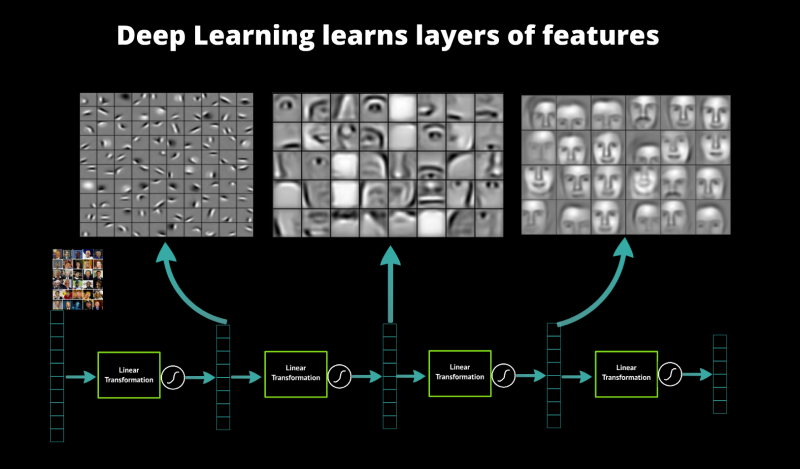
\includegraphics[width=0.85\linewidth]{lectures/01-a/dl_features.png}
% Figure from: https://www.datasciencecentral.com/profiles/blogs/a-primer-on-deep-learning
\caption{In the figure above we see how the layers closer to the input of the network are more abstract, and that those closer to the final layer are most concrete and interpretable.}
\label{fig:deep-learning-hierarchical-features}
\end{figure}

In a neural network, we feed the output of one layer onto the input of the next.
Layers are composed of linear transformations followed by non-linear activation functions.
Altogether, this system allows the network to learn the non-linear features of interest.

Hierarchical feature representations are intuitive for many domains, as our world is compositional (the whole is often a function of its parts).
For example, consider the following domains:
\begin{itemize}
    \item \textbf{Image recognition}: Pixels compose edges, which compose ``textons'' (i.e., multi-edge shapes), which compose motifs, which compose parts, which finally compose whole objects.
    Algorithms may learn to understand what an object looks like by learning a function mapping from pixels to a slightly higher level representation such as edges, then to textons, etc., until a high enough level representation is formed to represent whole objects.
    Indeed, there is evidence from neuroscience that the visual cortex represents objects in such a hierarchical manner in animals.

    \item \textbf{Language}: Language is inherently compositional as well.
    The meaning of a book is a composition of the meanings of its chapters, then paragraphs, then sentences, then phrases, then words (then even characters).
    While not all language is compositional (a ``heavy accent'' has nothing to do with weight), it often is, as language is how humans represent the world which is often compositional.

    \item \textbf{Speech}: In speech, a sample composes a band, which composes a sound, which compose phones, then phonemes, then whole words and sentences.
    The capacity for each component of this hierarchy in speech is what enables hierarchical models to represent very high-level features of sound by simply forming consecutively higher representations over what is ultimately a series of bytes.
\end{itemize}

%%%%%%%%%%%%%%%%%%%%%%%%%%%%%%%%%%%%%%%%%%
\part{Practice}\label{prt:practice}
%%%%%%%%%%%%%%%%%%%%%%%%%%%%%%%%%%%%%%%%%%
\chapter{Tensor Transformations}
% Authors: Dustin Godevais , Reuben Juster, Yi Li,. 2/5/18.

The following sections summarize and visualize how you can transform data represented in matrix form. 
Input data can be defined as a matrix with the $i^{th}$ row corresponding to the $i^{th}$ data point and each additional columns representing a new dimension of the data.
$\matr{X}$ in the below examples is an input matrix with 1000 data points and two dimensions whose values are standard normally distributed. 
In the following figures, data points are colored according to their original $x_{N,1}$  dimension violet to yellow for negative to positive values.

\[
\matr{X} =
\begin{bmatrix}
    x_{1,1} & x_{1,2} \\
    x_{2,1} & x_{2,2} \\
    x_{3,1} & x_{3,2} \\
    \vdots & \vdots  \\
    x_{1000,1} & x_{1000,2}
\end{bmatrix}
\]

\begin{figure}[H]
\begin{center}
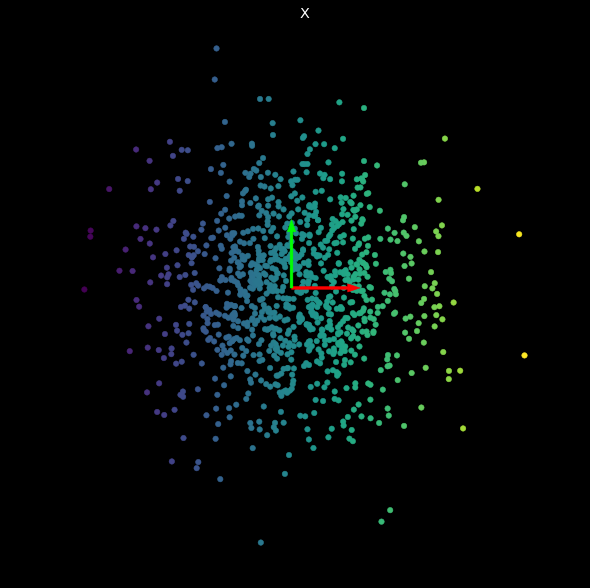
\includegraphics[width=200pt]{labs/01/images/standardnormal.png}
\end{center} 
\caption{Original $\matr{X}$ Visualized}
% \label{fig:mon}
\end{figure}

\section{Linear Transformations}
% Authors: Dustin Godevais , Reuben Juster, Yi Li,. 2/5/18.
There are several linear transformation that can be executed on $\matr{X}$ including:

\begin{itemize}
% \tightlist
\item
Rotation (\(\matr{U}\))

\item
Scaling \((s_1, s_2)\)

\item
Reflection (\(\matr{V}\))
\item
Shearing
\item
Translation
\end{itemize}

The product of the first three form weights as shown below.

\[
\matr{W} = \matr{U}
\begin{bmatrix}
    s_1 & 0 \\
    0 & s_2 
\end{bmatrix}
\matr{V}^\top
\]


\subsection{Rotation}
During rotation, each point is rotated about the origin by the indicated angle. 
The below equation populates $\matr{U}$ based on rotating points by \(\theta\) counter-clockwise.

\[
\matr{U} = 
\begin{bmatrix}
    \cos(\theta) & \sin(\theta)\\
    \sin(\theta) & -\cos(\theta)
\end{bmatrix}
\]

Keeping scaling and reflection constant, the below figure shows a set up points with different  \(\theta\)s .

\begin{figure}[H]
\begin{center}
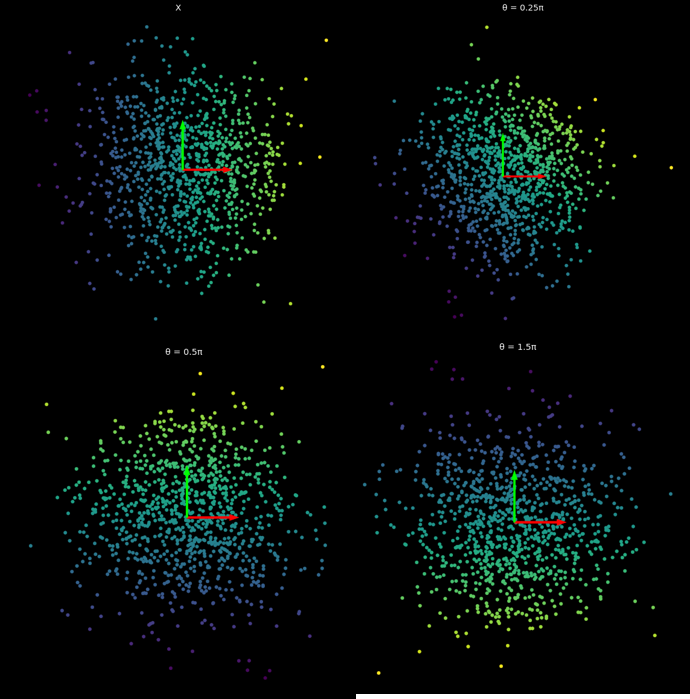
\includegraphics[width=300pt]{labs/01/images/Rotation.png}
\end{center} 
\caption{Rotation Visualized}
% \label{fig:mon}
\end{figure}
% \FloatBarrier


\subsection{Scaling}
Scaling the points expands or contracts the points about the origin. 
This controlled separately for each dimension by \(s_1\) and \(s_2\) .

\begin{figure}[H]
\begin{center}
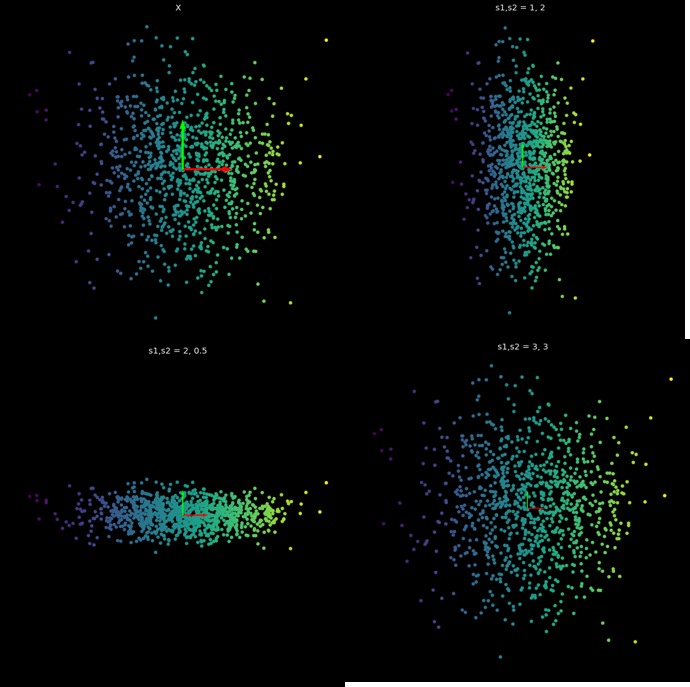
\includegraphics[width=300pt]{labs/01/images/Scaling.png}
\caption{Scaling Visualized}
% \label{fig:mon}
\end{center} 
\end{figure}
% \FloatBarrier


\subsection{Reflection}
Reflecting points projects them on the other side of a defined line that crosses the origin. 
The line that goes from the original point to the projected point is perpendicular to the defined line, and the intersection to the defined line is the midpoint.


\begin{figure}[H]
\begin{center}

\includegraphics[width=200pt]{labs/01/images/reflection_example.png}
\end{center} 
\caption{Reflection Defined}
% \label{fig:mon}
\end{figure}
% \FloatBarrier


\(\matr{V}\) can be defined by

\[
\matr{V} = 
\begin{bmatrix}
    \cos(2\theta) & \sin(2\theta)\\
    \sin(2\theta) & -\cos(2\theta)
\end{bmatrix}
\]

Where the defined line is \(x_2 = \tan(\theta) x_1 \)

\begin{figure}[H]
\begin{center}
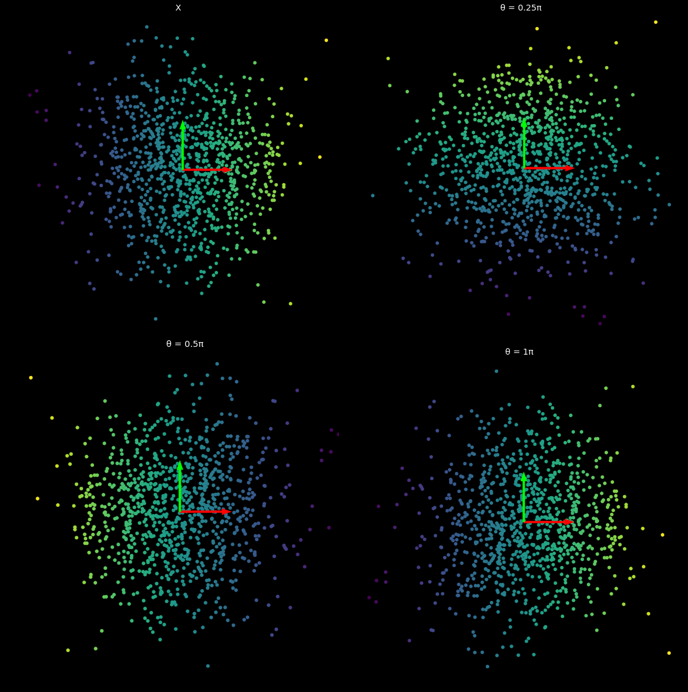
\includegraphics[width=400pt]{labs/01/images/Reflection.png}
\end{center} 
\caption{Reflection Visualized}
% \label{fig:mon}
\end{figure}
% \FloatBarrier

\subsection{Shearing}
Shearing points, which is separate from the weight calculation, shifting points in one dimension proportional to their value in the other dimension.

\(\matr{Y} = \matr{X}  \begin{bmatrix}
    1 & k\\
    0 & 1
\end{bmatrix} \) 
Shift points on the \(x_1\) dimension proportional to the \(x_2\) dimension

\(\matr{Y} = \matr{X}  \begin{bmatrix}
    1 & 0\\
    k & 1
\end{bmatrix} \)
Shift points on the \(x_2\) dimension proportional to the \(x_1\) dimension

\begin{figure}[H]
\begin{center}
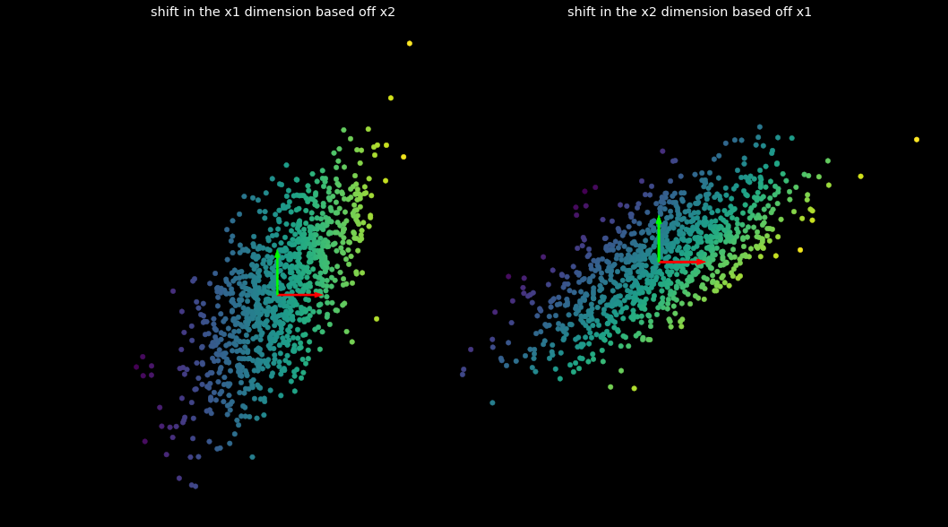
\includegraphics[width=400pt]{labs/01/images/shear.png}
\end{center} 
\caption{Shear Visualized}
% \label{fig:mon}
\end{figure}
% \FloatBarrier

\subsection{Translation}
The translation of points, which is separate from the weight calculations moves them uniforming in the direction indicated.

\[ \matr{Y} = \matr{X} 
+ \begin{bmatrix}
    1 & 1 \\
    1 & 1 \\
    1 & 1 \\
    \vdots & \vdots  \\
    1 & 1
\end{bmatrix}
\begin{bmatrix}
    t_1 & 0\\
    0 & t_2
\end{bmatrix} \] 
(Shift points left or right by \(t_1\) and up or down by  \(t_2\) dimension)

\begin{figure}[H]
\begin{center}
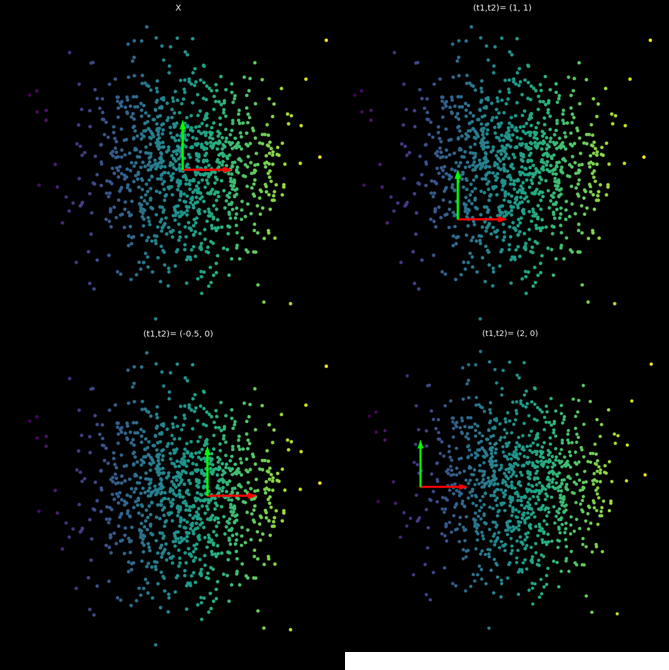
\includegraphics[width=400pt]{labs/01/images/translation.png}
\end{center} 
\caption{Translation Visualized}
% \label{fig:mon}
\end{figure}
% \FloatBarrier

\section{Non-Linear Transformations}
% Authors: Dustin Godevais , Reuben Juste, Yi Li,. 2/5/18.
Linear transformations are capable of altering data in many different ways, but linear transformations cannot curve data. 
That is where non-linear transformations come in. There are several types of non-linear transformations such as:

\begin{itemize}
% \tightlist
\item
Rectified linear unit (ReLU) - \(y = x_1\) if \(x_1 > 0\) else $0$ 
\item
Polynomial- \(y = x_1^2\) or \(y = x_1 x_2\)
\item
Step - \(y = 1\) if \(x > 0 \) else $0$ 

\end{itemize}

One of the most common non-linear transformations is the hyperbolic tangent, which in the context of 2D Tensors can be applied as below:
\[f(x) = \tanh(
\begin{bmatrix}
s & 0\\
0 & s
\end{bmatrix}
x)\]

This function first stretches out the points using scalar $s$ via scaling, then the hyperbolic tanget squashes the points into a square.
The larger $s$ is, the more points end up in the square.

\begin{figure}[H]
\begin{center}
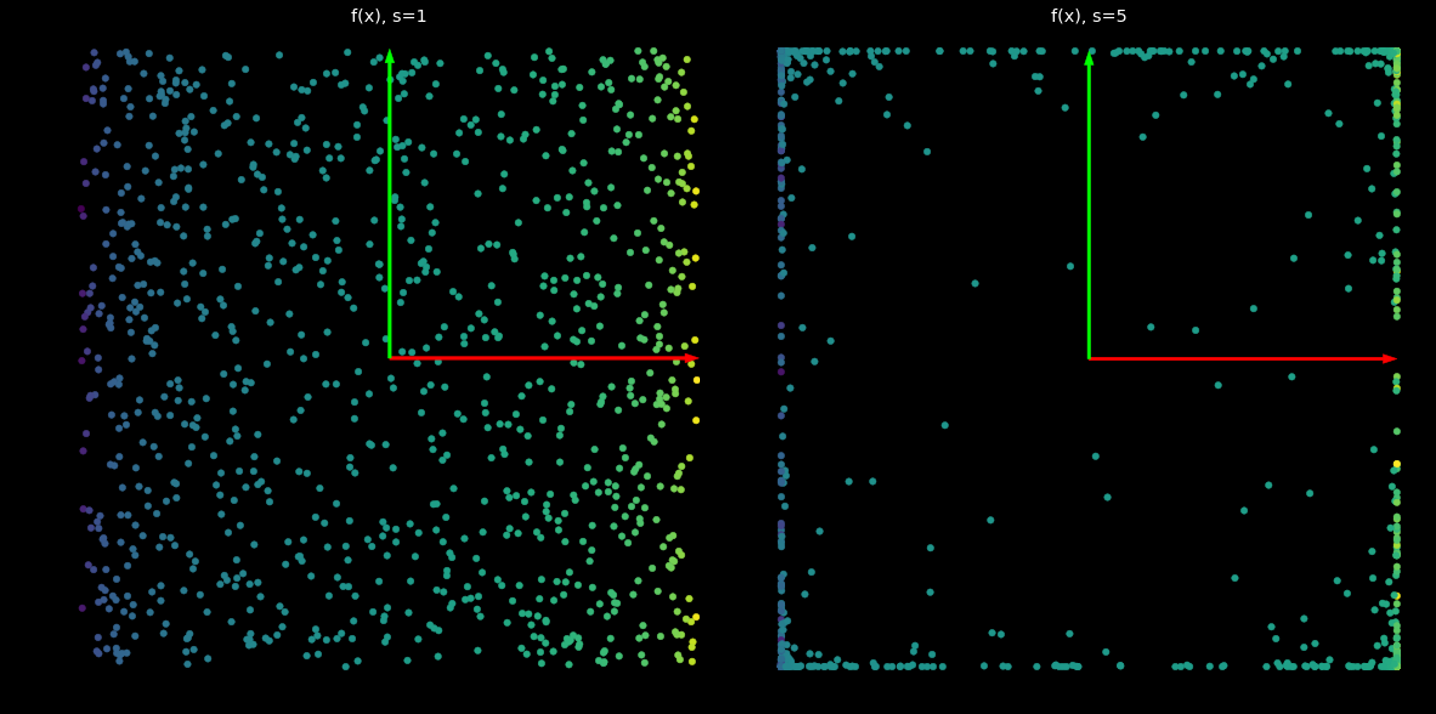
\includegraphics[width=400pt]{labs/01/images/tanh.png}
\end{center} 
\caption{Tanh in Isolation}
% \label{fig:mon}
\end{figure}
% \FloatBarrier

Tanh can create curved surfaces when it is sandwiched in-between two linear transformations in a three layer neural network.

\begin{figure}[H]
\begin{center}
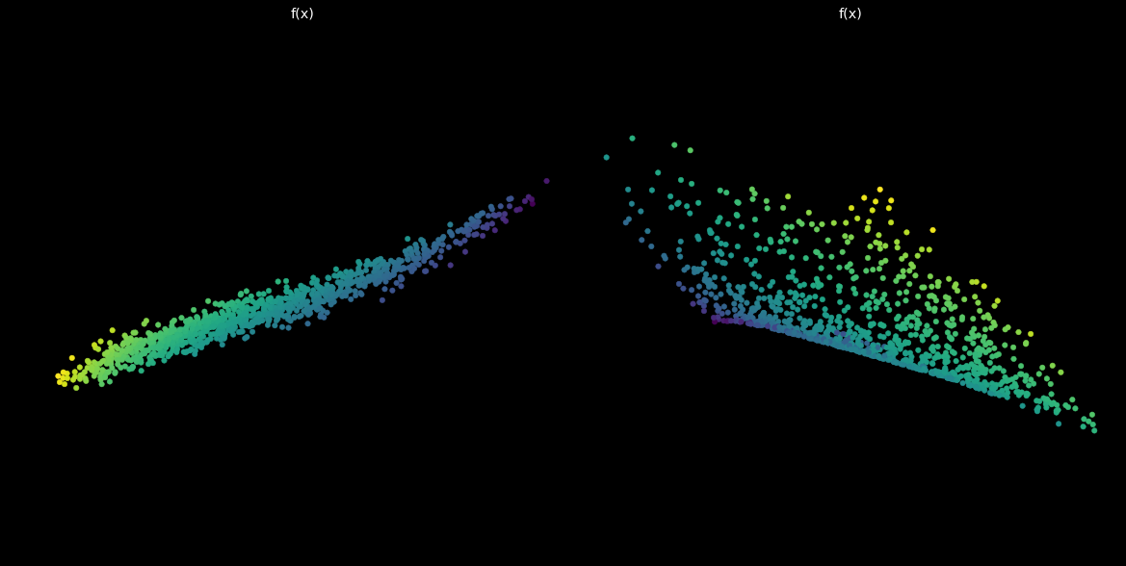
\includegraphics[width=400pt]{labs/01/images/tanh_sandwich.png}
\end{center} 
\caption{Tanh In-Between Two Linear Layers}
% \label{fig:mon}
\end{figure}
% \FloatBarrier

%%%%%%%%%%%%%%%%%%%%%%%%%%%%%%%%%%%%%%%%%%
\part{Coding}\label{prt:coding}
%%%%%%%%%%%%%%%%%%%%%%%%%%%%%%%%%%%%%%%%%%
\chapter{Introduction to \emph{PyTorch} and \texttt{Tensor}s}
% Authors: Dustin Godevais , Reuben Juste, Yi Li,. 2/5/18.
    \section{What is \emph{PyTorch}?}\label{what-is-pytorch}
    % Authors: Dustin Godevais , Reuben Juste, Yi Li,. 2/5/18.
    \emph{PyTorch} is a Python based scientific computing package targeting on two sets of audiences:

   
\begin{itemize}
% \tightlist
\item
  Tensorial library that uses the power of GPUs
\item
  A deep learning research platform that provides maximum flexibility
  and speed
\end{itemize}

    
     \begin{Verbatim}[commandchars=\\\{\}]
{\color{incolor}In [{\color{incolor}1}]:} \PY{k+kn}{import} \PY{n+nn}{torch}
\end{Verbatim}

    \section{Getting help in Jupyter}\label{getting-help-in-jupyter}
    % Authors: Dustin Godevais , Reuben Juste, Yi Li,. 2/5/18.

    
%\subsection*{Jupyter Tips}
    \href{https://jupyter.org/}{Jupyter Notebook} is a common Integrated Development Environment (IDE) for deep learning. There are a few commands specific to Jupyter Notebook that are helpful for coding.   
        \subsection{Using tab}
        Tab will list all available functions, while shift + tab will open the documentation.

        \subsection{Using ?}
        \begin{Verbatim}[commandchars=\\\{\}]
{\color{incolor}In [{\color{incolor}2}]:} \PY{c+c1}{\PYZsh{} Open the documentation, same as \PYZlt{}shift\PYZgt{} + \PYZlt{}tab\PYZgt{} on \PYZsq{}torch.nn.Module()\PYZsq{}}
         torch.nn.Module\PY{o}{?}
\end{Verbatim}


    \begin{Verbatim}[commandchars=\\\{\}]
{\color{incolor}In [{\color{incolor}3}]:} \PY{c+c1}{\PYZsh{} See the source code of all functions being executed in the Module}
         torch.nn.Module\PY{o}{??}
\end{Verbatim}
        
\subsection{Dropping to Bash}
\begin{Verbatim}[commandchars=\\\{\}]
{\color{incolor}In [{\color{incolor}4}]:} \PY{c+c1}{\PYZsh{} List all the files in the current directory}
         \PY{o}{!}ls \PYZhy{}lh 
\end{Verbatim}

\begin{Verbatim}[commandchars=\\\{\}]
{\color{incolor}In [{\color{incolor}5}]:} \PY{c+c1}{\PYZsh{} Getting some general help}
         \PY{o}{\PYZpc{}}\PY{k}{magic} 
\end{Verbatim}

\section{Tensors}\label{tensors}   
% Authors: Dustin Godevais , Reuben Juste, Yi Li,. 2/5/18.
A tensor is a n-dimensional array, \emph{PyTorch} provides functions for operating on Tensors like numpy does for arrays.
\begin{Verbatim}[commandchars=\\\{\}]
{\color{incolor}In [{\color{incolor}6}]:} \PY{c+c1}{\PYZsh{} Generate a tensor of size 2x3x4}
         \PY{n}{t} \PY{o}{=} \PY{n}{torch}\PY{o}{.}\PY{n}{Tensor}\PY{p}{(}\PY{l+m+mi}{2}\PY{p}{,} \PY{l+m+mi}{3}\PY{p}{,} \PY{l+m+mi}{4}\PY{p}{)}
         \PY{n+nb}{type}\PY{p}{(}\PY{n}{t}\PY{p}{)} 
\end{Verbatim}


\begin{Verbatim}[commandchars=\\\{\}]
{\color{outcolor}Out[{\color{outcolor}6}]:} torch.Tensor
\end{Verbatim}
            
\begin{Verbatim}[commandchars=\\\{\}]
{\color{incolor}In [{\color{incolor}7}]:} \PY{c+c1}{\PYZsh{} Get the size of the tensor}
         \PY{n}{t}\PY{o}{.}\PY{n}{size}\PY{p}{(}\PY{p}{)} 
\end{Verbatim}


\begin{Verbatim}[commandchars=\\\{\}]
{\color{outcolor}Out[{\color{outcolor}7}]:} torch.Size([2, 3, 4])
\end{Verbatim}
            
\begin{Verbatim}[commandchars=\\\{\}]
{\color{incolor}In [{\color{incolor}8}]:} \PY{c+c1}{\PYZsh{} Get the dimension of the tensor, for example, 1 for vectors, 2 for matrices}
         \PY{n}{t}\PY{o}{.}\PY{n}{dim}\PY{p}{(}\PY{p}{)} 
\end{Verbatim}


\begin{Verbatim}[commandchars=\\\{\}]
{\color{outcolor}Out[{\color{outcolor}8}]:} 3
\end{Verbatim}
            
\begin{Verbatim}[commandchars=\\\{\}]
{\color{incolor}In [{\color{incolor}9}]:} \PY{c+c1}{\PYZsh{} Total number of elements in the tensor}
         \PY{n}{t}\PY{o}{.}\PY{n}{numel}\PY{p}{(}\PY{p}{)} 
\end{Verbatim}


\begin{Verbatim}[commandchars=\\\{\}]
{\color{outcolor}Out[{\color{outcolor}9}]:} 24
\end{Verbatim}
 
Note: Mind the underscore! 
Any operation that mutates a tensor in-place is post-fixed with an underscore. 
The in-place replacement will change the object. It is encouraged to perform operations in-place to optimize usage of memory.
            
\begin{Verbatim}[commandchars=\\\{\}]
{\color{incolor}In [{\color{incolor}10}]:} 
         \PY{n}{t}\PY{o}{.}\PY{n}{random\PYZus{}}\PY{p}{(}\PY{l+m+mi}{10}\PY{p}{)} 
\end{Verbatim}


\begin{Verbatim}[commandchars=\\\{\}]
{\color{outcolor}Out[{\color{outcolor}10}]:} tensor([[[4., 6., 2., 4.],
                  [8., 2., 6., 9.],
                  [1., 4., 9., 9.]],
         
                 [[8., 5., 5., 5.],
                  [4., 1., 1., 7.],
                  [4., 4., 6., 9.]]])
\end{Verbatim}
            
\begin{Verbatim}[commandchars=\\\{\}]
{\color{incolor}In [{\color{incolor}11}]:} \PY{n}{r} \PY{o}{=} \PY{n}{torch}\PY{o}{.}\PY{n}{Tensor}\PY{p}{(}\PY{n}{t}\PY{p}{)}
         \PY{c+c1}{\PYZsh{} This resizes the tensor permanently}
         \PY{n}{r}\PY{o}{.}\PY{n}{resize\PYZus{}}\PY{p}{(}\PY{l+m+mi}{3}\PY{p}{,} \PY{l+m+mi}{8}\PY{p}{)}  
         \PY{n}{r}
\end{Verbatim}


\begin{Verbatim}[commandchars=\\\{\}]
{\color{outcolor}Out[{\color{outcolor}11}]:} tensor([[4., 6., 2., 4., 8., 2., 6., 9.],
                 [1., 4., 9., 9., 8., 5., 5., 5.],
                 [4., 1., 1., 7., 4., 4., 6., 9.]])
\end{Verbatim}
            
\begin{Verbatim}[commandchars=\\\{\}]
{\color{incolor}In [{\color{incolor}12}]:} \PY{c+c1}{\PYZsh{} Replace all element in r with 0\PYZsq{}s}
         \PY{n}{r}\PY{o}{.}\PY{n}{zero\PYZus{}}\PY{p}{(}\PY{p}{)} 
\end{Verbatim}


\begin{Verbatim}[commandchars=\\\{\}]
{\color{outcolor}Out[{\color{outcolor}12}]:} tensor([[0., 0., 0., 0., 0., 0., 0., 0.],
                 [0., 0., 0., 0., 0., 0., 0., 0.],
                 [0., 0., 0., 0., 0., 0., 0., 0.]])
\end{Verbatim}
            
\begin{Verbatim}[commandchars=\\\{\}]
{\color{incolor}In [{\color{incolor}13}]:} \PY{n}{t}
\end{Verbatim}


\begin{Verbatim}[commandchars=\\\{\}]
{\color{outcolor}Out[{\color{outcolor}13}]:} tensor([[[0., 0., 0., 0.],
                  [0., 0., 0., 0.],
                  [0., 0., 0., 0.]],
         
                 [[0., 0., 0., 0.],
                  [0., 0., 0., 0.],
                  [0., 0., 0., 0.]]])
\end{Verbatim}
         
            
\begin{Verbatim}[commandchars=\\\{\}]
{\color{incolor}In [{\color{incolor}14}]:} \PY{c+c1}{\PYZsh{} Make a copy of r rather than replace r. }
         \PY{n}{s} \PY{o}{=} \PY{n}{r}\PY{o}{.}\PY{n}{clone}\PY{p}{(}\PY{p}{)} 
\end{Verbatim}
 Q: Why don\PYZsq{}t we always do this? \\
 A: It's time-consuming due to memory allocation, especially when we are training a neural network.  


\begin{Verbatim}[commandchars=\\\{\}]
{\color{incolor}In [{\color{incolor}15}]:} \PY{c+c1}{\PYZsh{} In\PYZhy{}place fill of 1\PYZsq{}s}
         \PY{n}{s}\PY{o}{.}\PY{n}{fill\PYZus{}}\PY{p}{(}\PY{l+m+mi}{1}\PY{p}{)} 
         \PY{n}{s}
\end{Verbatim}


\begin{Verbatim}[commandchars=\\\{\}]
{\color{outcolor}Out[{\color{outcolor}15}]:} tensor([[1., 1., 1., 1., 1., 1., 1., 1.],
                 [1., 1., 1., 1., 1., 1., 1., 1.],
                 [1., 1., 1., 1., 1., 1., 1., 1.]])
\end{Verbatim}
            
\begin{Verbatim}[commandchars=\\\{\}]
{\color{incolor}In [{\color{incolor}16}]:} \PY{c+c1}{\PYZsh{} Because we cloned r, even though we did an in\PYZhy{}place operation, this doesn\PYZsq{}t affect r}
         \PY{n}{r} 
\end{Verbatim}


\begin{Verbatim}[commandchars=\\\{\}]
{\color{outcolor}Out[{\color{outcolor}16}]:} tensor([[0., 0., 0., 0., 0., 0., 0., 0.],
                 [0., 0., 0., 0., 0., 0., 0., 0.],
                 [0., 0., 0., 0., 0., 0., 0., 0.]])
\end{Verbatim}
          

\subsection{Vectors: 1D Tensor}
\begin{Verbatim}[commandchars=\\\{\}]
{\color{incolor}In [{\color{incolor}17}]:} \PY{n}{v} \PY{o}{=} \PY{n}{torch}\PY{o}{.}\PY{n}{Tensor}\PY{p}{(}\PY{p}{[}\PY{l+m+mi}{1}\PY{p}{,} \PY{l+m+mi}{2}\PY{p}{,} \PY{l+m+mi}{3}\PY{p}{,} \PY{l+m+mi}{4}\PY{p}{]}\PY{p}{)}
         \PY{n}{w} \PY{o}{=} \PY{n}{torch}\PY{o}{.}\PY{n}{Tensor}\PY{p}{(}\PY{p}{[}\PY{l+m+mi}{1}\PY{p}{,} \PY{l+m+mi}{0}\PY{p}{,} \PY{l+m+mi}{2}\PY{p}{,} \PY{l+m+mi}{0}\PY{p}{]}\PY{p}{)}
         \PY{c+c1}{\PYZsh{} Element\PYZhy{}wise multiplication}
         \PY{n}{v} \PY{o}{*} \PY{n}{w} 
\end{Verbatim}


\begin{Verbatim}[commandchars=\\\{\}]
{\color{outcolor}Out[{\color{outcolor}17}]:} tensor([1., 0., 6., 0.])
\end{Verbatim}
            
\begin{Verbatim}[commandchars=\\\{\}]
{\color{incolor}In [{\color{incolor}18}]:} \PY{c+c1}{\PYZsh{} Scalar product: 1*1 + 2*0 + 3*2 + 4*0}
         \PY{n}{v} \PY{o}{@} \PY{n}{w} 
\end{Verbatim}


\begin{Verbatim}[commandchars=\\\{\}]
{\color{outcolor}Out[{\color{outcolor}18}]:} tensor(7.)
\end{Verbatim}
            
\begin{Verbatim}[commandchars=\\\{\}]
{\color{incolor}In [{\color{incolor}19}]:} \PY{n}{x} \PY{o}{=} \PY{n}{torch}\PY{o}{.}\PY{n}{Tensor}\PY{p}{(}\PY{l+m+mi}{5}\PY{p}{)}\PY{o}{.}\PY{n}{random\PYZus{}}\PY{p}{(}\PY{l+m+mi}{10}\PY{p}{)}
         \PY{n}{x}
\end{Verbatim}


\begin{Verbatim}[commandchars=\\\{\}]
{\color{outcolor}Out[{\color{outcolor}19}]:} tensor([6., 0., 5., 9., 7.])
\end{Verbatim}
            
   

\begin{Verbatim}[commandchars=\\\{\}]
{\color{incolor}In [{\color{incolor}20}]:} \PY{c+c1}{\PYZsh{} Extract sub\PYZhy{}Tensor [from:to)}
         \PY{n}{x}\PY{p}{[}\PY{l+m+mi}{1}\PY{p}{:}\PY{l+m+mi}{2} \PY{o}{+} \PY{l+m+mi}{1}\PY{p}{]} 
\end{Verbatim}


\begin{Verbatim}[commandchars=\\\{\}]
{\color{outcolor}Out[{\color{outcolor}20}]:} tensor([0., 5.])
\end{Verbatim}
       
Note: torch.arange gives only integers. Use torch.arange(1, 4 + 1, dtype = torch.float) to generate float numbers.      
            
\begin{Verbatim}[commandchars=\\\{\}]
{\color{incolor}In [{\color{incolor}21}]:} \PY{c+c1}{\PYZsh{} Create a tensor with integers ranging from 1 to 5, excluding 5}
         \PY{n}{v} \PY{o}{=} \PY{n}{torch}\PY{o}{.}\PY{n}{arange}\PY{p}{(}\PY{l+m+mi}{1}\PY{p}{,} \PY{l+m+mi}{4} \PY{o}{+} \PY{l+m+mi}{1}\PY{p}{)} 
         \PY{n}{v} 
\end{Verbatim}


\begin{Verbatim}[commandchars=\\\{\}]
{\color{outcolor}Out[{\color{outcolor}21}]:} tensor([1, 2, 3, 4])
\end{Verbatim}
\subsection{Matrices: 2D Tensor}
\begin{Verbatim}[commandchars=\\\{\}]
{\color{incolor}In [{\color{incolor}22}]:} \PY{c+c1}{\PYZsh{} Create a 2x4 tensor}
         \PY{n}{m} \PY{o}{=} \PY{n}{torch}\PY{o}{.}\PY{n}{Tensor}\PY{p}{(}\PY{p}{[}\PY{p}{[}\PY{l+m+mi}{2}\PY{p}{,} \PY{l+m+mi}{5}\PY{p}{,} \PY{l+m+mi}{3}\PY{p}{,} \PY{l+m+mi}{7}\PY{p}{]}\PY{p}{,}
                           \PY{p}{[}\PY{l+m+mi}{4}\PY{p}{,} \PY{l+m+mi}{2}\PY{p}{,} \PY{l+m+mi}{1}\PY{p}{,} \PY{l+m+mi}{9}\PY{p}{]}\PY{p}{]}\PY{p}{)} 
\end{Verbatim}
            
\begin{Verbatim}[commandchars=\\\{\}]
{\color{incolor}In [{\color{incolor}23}]:} \PY{c+c1}{\PYZsh{} Indexing column 0, row 2, it returns a 0\PYZhy{}dimensional tensor, which is a scalar. Or m[0,2]}
          \PY{n}{m}\PY{p}{[}\PY{l+m+mi}{0}\PY{p}{]}\PY{p}{[}\PY{l+m+mi}{2}\PY{p}{]} 
\end{Verbatim}


\begin{Verbatim}[commandchars=\\\{\}]
{\color{outcolor}Out[{\color{outcolor}23}]:} tensor(3.)
\end{Verbatim}
            
\begin{Verbatim}[commandchars=\\\{\}]
{\color{incolor}In [{\color{incolor}24}]:} \PY{c+c1}{\PYZsh{} Extract the single value in the scalar}
          \PY{n}{m}\PY{p}{[}\PY{l+m+mi}{0}\PY{p}{,}\PY{l+m+mi}{2}\PY{p}{]}\PY{o}{.}\PY{n}{item}\PY{p}{(}\PY{p}{)} 
\end{Verbatim}
Q: Why won't we extract value always? \\
A: A tensor will remember who is the parent, so we need to use tensor rather than just the scalar number when we perform back propagation during training a neural network.

\begin{Verbatim}[commandchars=\\\{\}]
{\color{outcolor}Out[{\color{outcolor}24}]:} 3.0
\end{Verbatim}
            
\begin{Verbatim}[commandchars=\\\{\}]
{\color{incolor}In [{\color{incolor}25}]:} \PY{c+c1}{\PYZsh{} Indexing column 1, all rows (returns size 2)}
          \PY{n}{m}\PY{p}{[}\PY{p}{:}\PY{p}{,} \PY{l+m+mi}{1}\PY{p}{]} 
\end{Verbatim}


\begin{Verbatim}[commandchars=\\\{\}]
{\color{outcolor}Out[{\color{outcolor}25}]:} tensor([5., 2.])
\end{Verbatim}
            
\begin{Verbatim}[commandchars=\\\{\}]
{\color{incolor}In [{\color{incolor}26}]:} \PY{c+c1}{\PYZsh{} Add one more bracket inside will add an extra dimension, now it\PYZsq{}s a 2 * 1 matrix }
          \PY{n}{m}\PY{p}{[}\PY{p}{:}\PY{p}{,} \PY{p}{[}\PY{l+m+mi}{1}\PY{p}{]}\PY{p}{]} 
\end{Verbatim}


\begin{Verbatim}[commandchars=\\\{\}]
{\color{outcolor}Out[{\color{outcolor}26}]:} tensor([[5.],
                  [2.]])
\end{Verbatim}

            
\begin{Verbatim}[commandchars=\\\{\}]
{\color{incolor}In [{\color{incolor}27}]:} \PY{c+c1}{\PYZsh{} Same as m.transpose(0, 1)}
          \PY{n}{m}\PY{o}{.}\PY{n}{t}\PY{p}{(}\PY{p}{)} 
\end{Verbatim}
Note: We can specify dimensions dimensions we want to swap using m.transpose(c1,c2) when we have many dimensions.

\begin{Verbatim}[commandchars=\\\{\}]
{\color{outcolor}Out[{\color{outcolor}27}]:} tensor([[2., 4.],
                  [5., 2.],
                  [3., 1.],
                  [7., 9.]])
\end{Verbatim}
            
\begin{Verbatim}[commandchars=\\\{\}]
{\color{incolor}In [{\color{incolor}28}]:} \PY{c+c1}{\PYZsh{} Create tensor from 3 to 8, with each having a space of 1}
          \PY{n}{torch}\PY{o}{.}\PY{n}{arange}\PY{p}{(}\PY{l+m+mf}{3.}\PY{p}{,} \PY{l+m+mi}{8} \PY{o}{+} \PY{l+m+mi}{1}\PY{p}{)} 
\end{Verbatim}


\begin{Verbatim}[commandchars=\\\{\}]
{\color{outcolor}Out[{\color{outcolor}28}]:} tensor([3., 4., 5., 6., 7., 8.])
\end{Verbatim}
            
\begin{Verbatim}[commandchars=\\\{\}]
{\color{incolor}In [{\color{incolor}29}]:} \PY{c+c1}{\PYZsh{} returns a 1D tensor of steps equally spaced points between start=3, end=8 and steps=20}
          \PY{n}{torch}\PY{o}{.}\PY{n}{linspace}\PY{p}{(}\PY{l+m+mi}{3}\PY{p}{,} \PY{l+m+mi}{8}\PY{p}{,} \PY{l+m+mi}{20}\PY{p}{)}\PY{o}{.}\PY{n}{view}\PY{p}{(}\PY{l+m+mi}{1}\PY{p}{,} \PY{o}{\PYZhy{}}\PY{l+m+mi}{1}\PY{p}{)} 
\end{Verbatim}


\begin{Verbatim}[commandchars=\\\{\}]
{\color{outcolor}Out[{\color{outcolor}29}]:} tensor([[3.0000, 3.2632, 3.5263, 3.7895, 4.0526, 4.3158, 4.5789, 4.8421, 5.1053,
                   5.3684, 5.6316, 5.8947, 6.1579, 6.4211, 6.6842, 6.9474, 7.2105, 7.4737,
                   7.7368, 8.0000]])
\end{Verbatim}
            
\begin{Verbatim}[commandchars=\\\{\}]
{\color{incolor}In [{\color{incolor}30}]:} \PY{c+c1}{\PYZsh{} Create a tensor filled with 0\PYZsq{}s torch.ones() will create a tensor filled with 1\PYZsq{}s.}
          \PY{n}{torch}\PY{o}{.}\PY{n}{zeros}\PY{p}{(}\PY{l+m+mi}{3}\PY{p}{,} \PY{l+m+mi}{5}\PY{p}{)} 
\end{Verbatim}


\begin{Verbatim}[commandchars=\\\{\}]
{\color{outcolor}Out[{\color{outcolor}30}]:} tensor([[0., 0., 0., 0., 0.],
                  [0., 0., 0., 0., 0.],
                  [0., 0., 0., 0., 0.]])
\end{Verbatim}
            
\begin{Verbatim}[commandchars=\\\{\}]
{\color{incolor}In [{\color{incolor}31}]:} \PY{c+c1}{\PYZsh{} Create a tensor with the diagonal filled with 1}
          \PY{n}{torch}\PY{o}{.}\PY{n}{eye}\PY{p}{(}\PY{l+m+mi}{3}\PY{p}{)}
\end{Verbatim}


\begin{Verbatim}[commandchars=\\\{\}]
{\color{outcolor}Out[{\color{outcolor}31}]:} tensor([[1., 0., 0.],
                  [0., 1., 0.],
                  [0., 0., 1.]])
\end{Verbatim}
\subsection{Images: 3D Tensor}
Q: Why would we use 4D Tensors while training convolutional neural networks?\\
A: Images are 3D Tensors with dimensions channels, height, and width. We will use a stack of multiple images to form a 4-dimensional tensor.


\section{References}
% Authors: Dustin Godevais , Reuben Juste, Yi Li,. 2/5/18.
\begin{itemize}
\tightlist
\item
\href{https://www.technologyuk.net/mathematics/algebra/matrices-as-transformations.shtml}{https://www.technologyuk.net/mathematics/algebra/matrices-as-transformations.shtml}
\item
\href{https://github.com/Atcold/pytorch-Deep-Learning-Minicourse/blob/master/01-tensor_tutorial.ipynb}{https://github.com/Atcold/pytorch-Deep-Learning-Minicourse/blob/master/01-tensor_tutorial.ipynb}
\item
\href{https://github.com/Atcold/pytorch-Deep-Learning-Minicourse/blob/master/02-space_stretching.ipynb}{https://github.com/Atcold/pytorch-Deep-Learning-Minicourse/blob/master/02-space_stretching.ipynb}
\end{itemize}
%%%%%%%%%%%%%%%%%%%%%%%%%%%%%%%%%%%%%%%%%%
\part{Applications}\label{prt:apps}
%%%%%%%%%%%%%%%%%%%%%%%%%%%%%%%%%%%%%%%%%%
%%%%%%%%%%%%%%%%%%%%%%%%%%%%%%%%%%%%%%%%%%
\part{Papers summary}\label{prt:papers}
%%%%%%%%%%%%%%%%%%%%%%%%%%%%%%%%%%%%%%%%%%

The end.  % \part needs to be followed by something.

\end{document}
